% INSTRUCTIONS:
% To compile this file, run "latex HW_example";  you need to do it TWICE
%    to get the cross-references (to equations, etc) to show correctly.
% Figures can be included as shown below.  If you don't have a figure,
%    comment out those lines using % signs at the beginning of each line,
%    or else just keep hitting RETURN when LaTeX gives an error message
%    saying that it can't find the figure file.
% Run "dvips HW_example.dvi" to make a Postscript file HW_example.ps,
%    and then "ps2pdf HW_example.ps" to make a PDF file HW_example.pdf.

\documentclass[12pt]{article}
\usepackage{graphicx,indentfirst}

\pagestyle{plain}
\baselineskip 18pt
\textwidth 6.5in
\textheight 7.8in
\oddsidemargin 0.1in
\evensidemargin 0.1in
\topmargin 0.3in

\newcommand{\be}{\begin{equation}}
\newcommand{\ee}{\end{equation}}
\newcommand{\reff}[1]{(\ref{#1})}


\begin{document}

\title{Computational Physics \\ Homework 2}
\author{Yi-Hsuan Hsu}
\date{09/18/2014}
\maketitle

\section{Problem 1}

Root-finding using bisection method, regula falsi, secant method, Newton's method. Observing error and convergence property in each method.

\subsection{Algorithms}

\subsubsection{Bisection Method}
\begin{figure}
	\begin{center}
		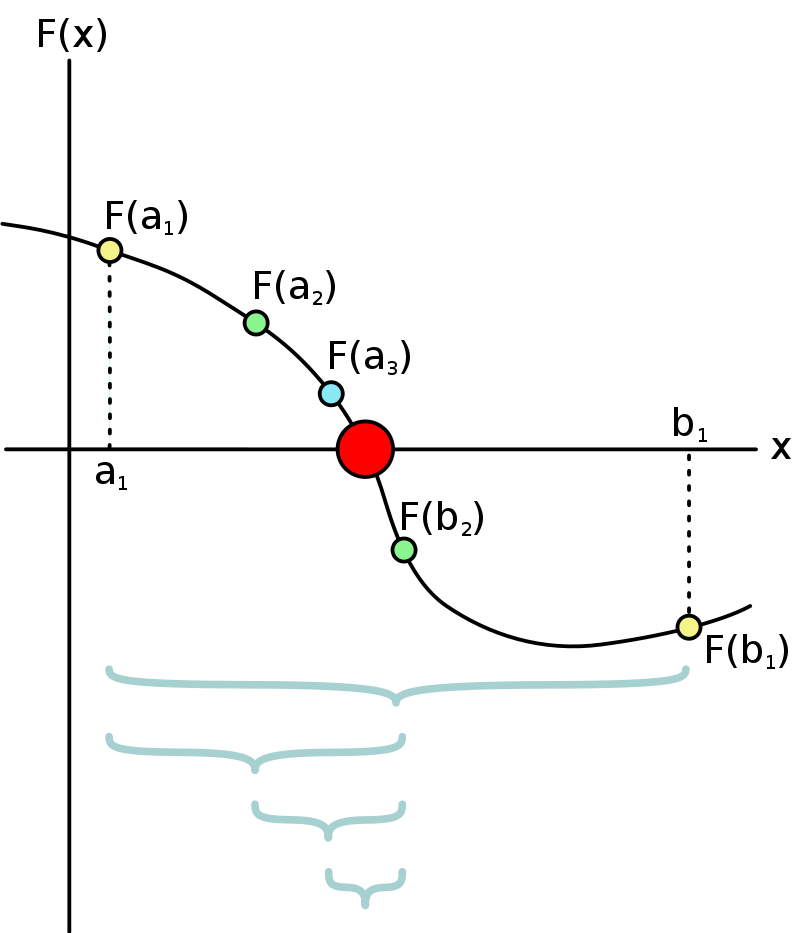
\includegraphics[width=0.4\textwidth]{bisection.png}
		\caption{In each iteration, take bisects of interval into subinterval. Make sure the left hand end times right hand end always get minus sign, we will approach close enough to root. Pic From Wiki}
		\label{fig1}
		
	\end{center}
\end{figure}

Bisection method take average point of an interval to form a new subinterval repeatly. In general, bisection method can alway find a root (given a contineous function with at least one root).
\begin{equation}
\epsilon_{n+1}=constant\times\epsilon_{n}^{m}
\end{equation}
where $\epsilon$ equal to difference of subinterval. Bisection method is convergent linearly, relatively slow compare to other method. 

\subsubsection{Regula Falsi Method}
Instead of average point as the end of subinterval, Regula Falsi using weight average in the fact that the closer $f(x_{n})$ to zero, the closer $x_{n}$ to the root.
\begin{equation}
w=[f(b_{n})\cdot a_{n} - f(a_{n})\cdot b_{n}]/[f(b_{n})-f(a_{n})]
\end{equation}
\begin{figure}
	\begin{center}
		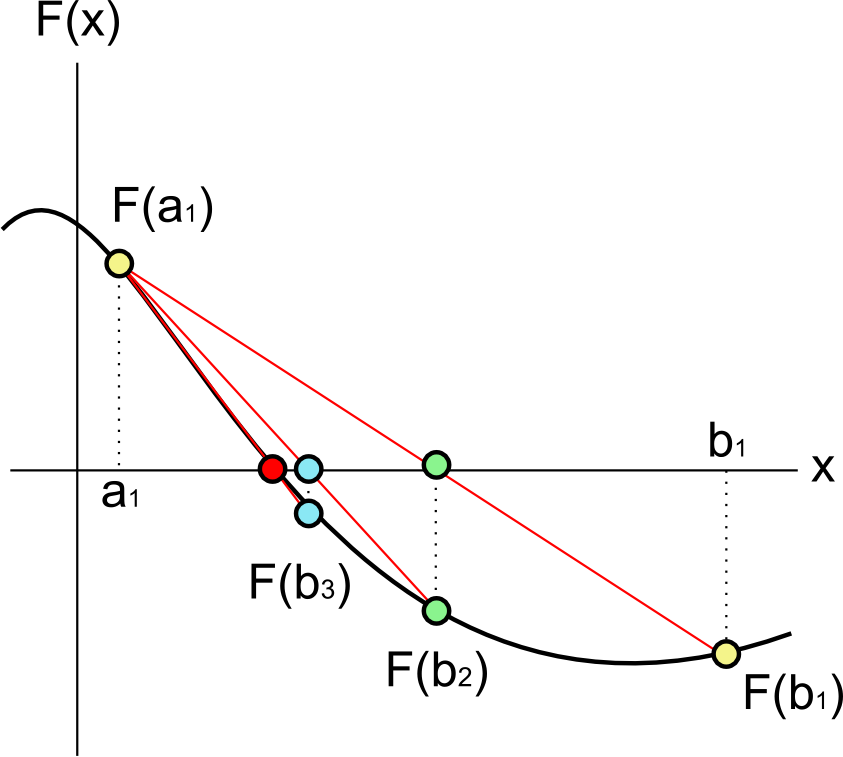
\includegraphics[width=0.4\textwidth]{Regula_falsi_method.png}
		\caption{Regula falsi method. Pic From Wiki}
		\label{fig2}
		
	\end{center}
\end{figure}

\subsubsection{Secant Method}
Secant method use a succession of roots of secant lines to better approximate a root of a function. We can estimate its convergence by following equation
\begin{equation}
\epsilon_{n+1}=const\times|\epsilon_{n}|^\phi
\end{equation}
where $\phi=1.618....$ is golden ratio. 
\subsubsection{Newton's Method}
From Taylor expansion of arbitrary function $f(x)$, we have
\begin{equation}
	f(x+\delta)\approx f(x)+f'(x)\delta+\frac{f''(x)}{2} \delta^2+...
\end{equation}
We can derive root finding procedure from an initial guess $x_{0}$ and derivative function $f'(x)$
\begin{equation}
	x_{n+1}=x_{n}-\frac{f(x_{n})}{f'(x_{n})}
\end{equation}
In my program, $f'(x)$ is defined
\begin{equation}
f'(x)=\frac{f(x-h)-f(x)}{h}
\end{equation}
$h=10^{-14}$.

The convergent rate of newton's method is quadratic. One can derive the recurrence relation for the deviations of the trial solution
\begin{equation}
\epsilon_{n+1}=-\epsilon^{2}\frac{f''(x)}{2f'(x)}
\end{equation}

\subsection{Description of program}
My program can divided to four part.

First, testing function and initial input. At the top of code is where I define testing function and give an initial interval and desired iteration. Initial interval can be assigned either single-float precision or double-float point precision.

Second part is root-finding part. Here I define root-finding function for each method and return $x_{n}$,$f(x_{n})$, $\epsilon_{n}(=|a_{n}-b_{n}|)$, $\delta_{n}(=|x_{n}-x^*|)$ in python list.

Third, main code throw initial value into functions. $if$ statement are applied to assure different sign of interval.

Forth, output each method in list. Draw picture of $\epsilon_{n}$ v.s. $n$ and $\delta_{n}$ v.s. $n$. Observing how different methods convergent and approach to exact solution.

\subsection{Sample output}
Take $sin(x)$ root-finding in $[3.0,3.5]$ as sample (see /out/func sin output.txt). 
Obviously, newton's method owns the fastest convergence rate. Only two iteration is used we approach the exact solution in machine's limit.
Regula falsi and secant are roughly convergent in the same rate. But secant method jumps less step than regular falsi does. Bisection method take over 30 steps to find the root within 1e-10 level.

Figure 3 illustrate clearly how $\epsilon_{n}$ and $\delta_{n}$ converge. We can see that bisection follows linear convergence while the other follow quadratic or higher order convergence. 

\begin{figure}[h]
	\begin{center}
		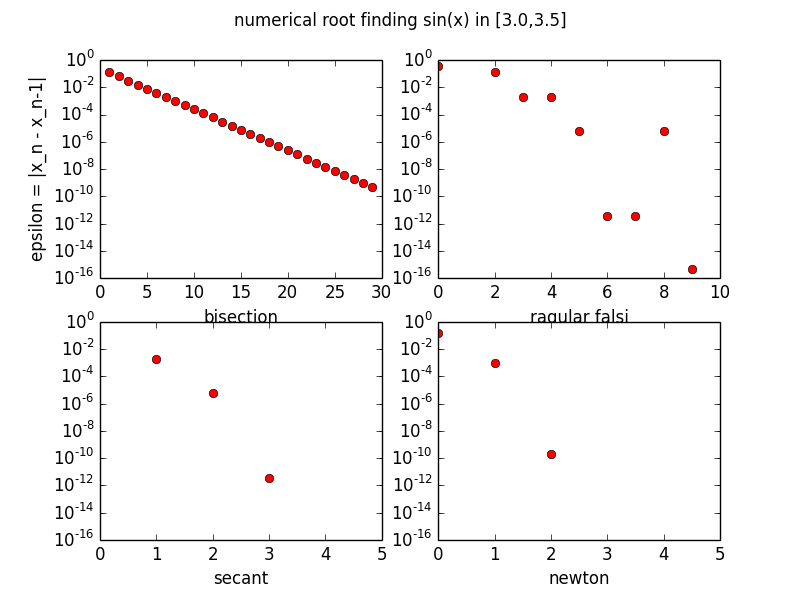
\includegraphics[width=0.5\textwidth]{eps_sin.png}
		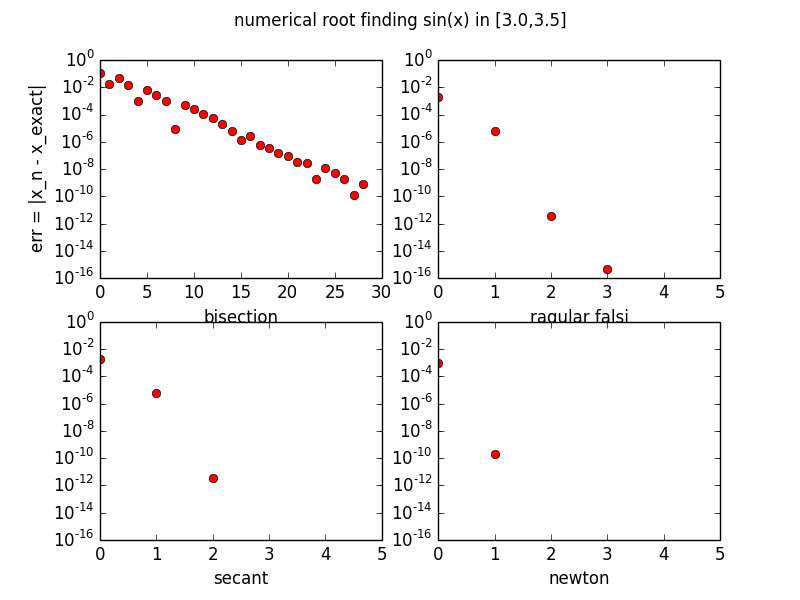
\includegraphics[width=0.5\textwidth]{err_sin.png}
		\caption{Sample output deisplay. Four different method are applied to find the root of $sin(x)$.
			Upper:y axis is $\epsilon_{n}$ ,x axis is iteration number. Lower: y axis is $\delta_{n}$, x axis is iteration number. }
		\label{fig3}
		
	\end{center}
\end{figure}

\subsection{Respond to Question}
\subsubsection{Question (b)}
	Figure 3 shows that $\epsilon_{n}$ do follow the way we expect. Although in Regula-falsi(R-F), secant and newton take only few iteration to find the root, we can still see their behavior clearly Except for small flactuation, bisection goes linearly, R-F and secant goes quadratic and newton in higher order. 
	
	Figure 4 compare the $\epsilon_{n}]$ of series iteration with different initial interval [3.0,3.5] and [3.0,4.5]. Obviously green dot is further than red dot, which implies initial condition or first guess affect efficiency very much, except for bisection method.

\begin{figure}[h]
	\begin{center}
		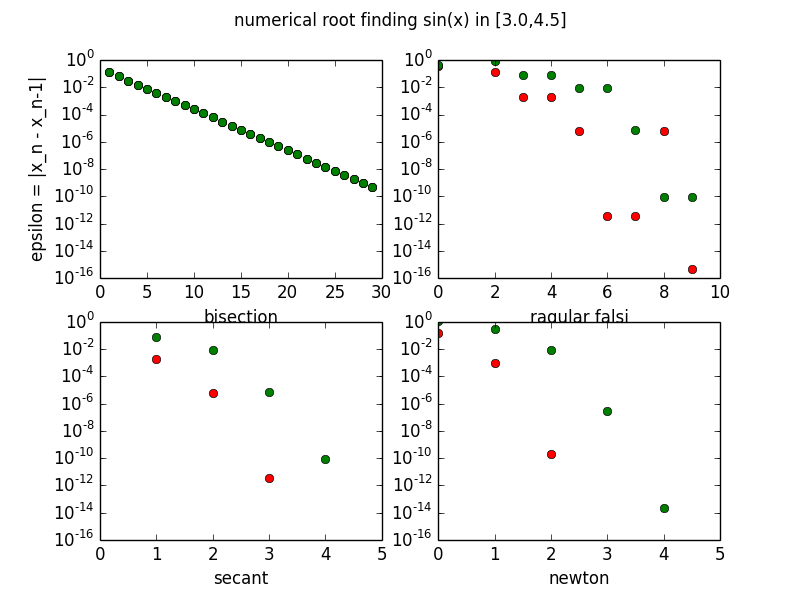
\includegraphics[width=0.5\textwidth]{figure_1.png}
		\caption{Series after initial interval $[3.0,3.5]$ are shown in red. Initial interval $[3.0,4.5]$ are shown is green.}
		\label{fig4}
		
	\end{center}
\end{figure}

\subsubsection{Question (c)}
	Figure 5 shows $\epsilon_{n}$ and $\delta_{n}$ for $sin(x)^{3}$ root-finding. Bisection still works well as it promised, even better than newton's method. Both bisection and newton converge linearly, which is not expected on newton's method. In the other hand, R-F and secant method seem "stuck". The some phenomena keep the same when the shorten the initial interval closer to exact answer. 
\begin{figure}[h]
\begin{center}
	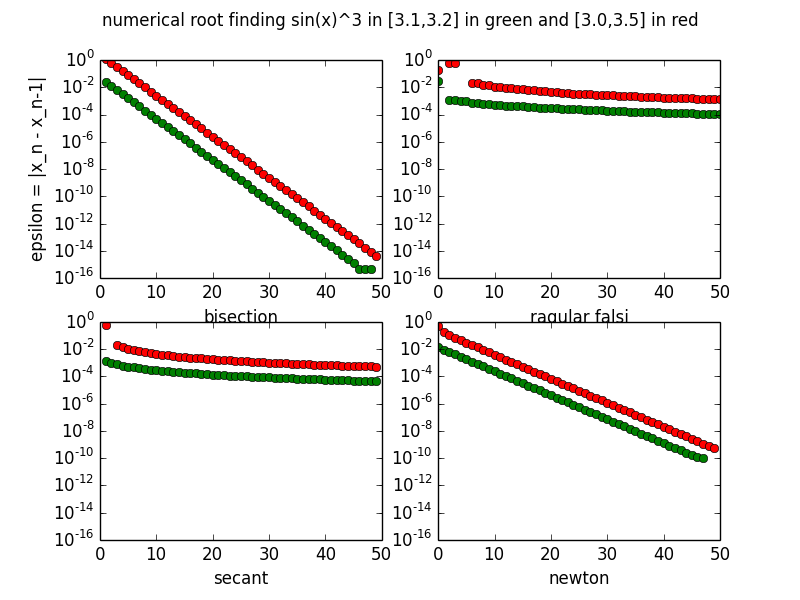
\includegraphics[width=0.5\textwidth]{eps_sin_tri_1.png}
	\caption{}
	\label{fig5}
\end{center}
\end{figure}

\subsubsection{Question (d)}
Again, take $sin(x)$ as an example. See $(/out/func sin output autostop.txt)$. Iteration series stop automatically. When I try on $f(x)=e^{x},1/x,x^{11},xe^{-\frac{1}{x^{2}}}$, the series goes to the left hand side or right hand side due to theres no root for such a function in arbitrary given interval in bisection and R-F method. In the other hand, series blows up in secant and newton method because bracket is broken.
\end{document}
